\documentclass{article}
\usepackage{graphicx}
\usepackage{amsmath}
\usepackage{booktabs}
\usepackage{siunitx}
\usepackage{float}
\usepackage[margin=1in]{geometry}

\title{Final Project 8.2 -- EE4725 Quasi Optical Systems\\
       Ka-band Satcom Dipole Array with Backing Reflector}
\author{Daniel Tyukov \\ Student Number: 5714699 \\ Microelectronics, TU Delft}
\date{April 2026}

\begin{document}

\maketitle

\tableofcontents
\newpage

%% ====================================================================
\section{System Specification}
%% ====================================================================

The objective is to design a planar phased array of printed dipoles backed by an infinite PEC reflector, to be embedded in an aircraft skin for Ku/Ka satellite-communication transmission. The array must operate over the Ka-band Satcom transmit window:
\begin{itemize}
\item Operating band: $f \in [\SI{27.5}{GHz},\;\SI{31}{GHz}]$ (\SI{3.5}{GHz}, $11.9\%$ fractional bandwidth)
\item Centre frequency: $f_c = \SI{29.25}{GHz}$, $\lambda_c = c/f_c = \SI{10.26}{mm}$, $k_0(f_c) = \SI{612.6}{rad/m}$
\item Free-space impedance $\zeta_0 = 120\pi\,\Omega$
\item In-band match target: $\Gamma_{\text{act}}(\mathrm{dB}) = 20\log_{10}\!\left|(Z_{\text{in,act}}-Z_L)/(Z_{\text{in,act}}+Z_L)\right| < \SI{-10}{dB}$
\end{itemize}

The free design parameters are the dipole length $l$, width $w$, the array periods $d_x,d_y$, the height $h$ of the dipole plane above the PEC, and the feed reference impedance $Z_L$.

%% ====================================================================
\section{Theory: Active Impedance with a Backing Reflector}
%% ====================================================================

\subsection{Image-theorem Green's function}

A horizontal electric dipole at height $z = h$ above a PEC plane at $z = 0$ has its image at $z = -h$ with reversed current direction (image theorem for tangential J above a PEC). Adding the field of the source and the image, the spectral $xx$-component of the dyadic Green's function evaluated at the source plane is
\begin{equation}\label{eq:Geff}
\boxed{\;\widetilde{G}^{ej}_{xx,\,\text{eff}}(k_x,k_y;h) \;=\; \widetilde{G}^{ej}_{xx,\,\text{FS}}(k_x,k_y)\,\bigl[1 - e^{-j 2 k_z h}\bigr]\;}
\end{equation}
with $\widetilde{G}^{ej}_{xx,\,\text{FS}} = -\zeta_0(k_0^2-k_x^2)/(2k_0 k_z)$ and the standard branch $k_z = -j\sqrt{-(k_0^2-k_x^2-k_y^2)}$ (real positive for propagating modes, $-j|\cdot|$ for evanescent). The reflector factor $|1 - e^{-j 2 k_z h}|^2 = 4\sin^2(k_z h)$ for propagating modes, and at broadside ($k_z = k_0$) it peaks at $4$ when $h = \lambda/4$. The same factor also exponentially attenuates the higher-order \emph{evanescent} Floquet modes (since $k_z = -j|k_z|$ there), suppressing the inductive reactance of the inter-cell mutual coupling that we observed in Assignment~5 for free-space arrays.

\subsection{Active input impedance}

After Galerkin projection on the entire-domain sinusoidal basis function used in Assignments~5--6 the active input impedance is the discrete Floquet sum
\begin{equation}\label{eq:Zact}
Z_{\text{in,act}}(\theta_0,\phi_0) \;=\; -\frac{1}{d_x d_y}\sum_{m_x,m_y}\widetilde{G}^{ej}_{xx,\,\text{eff}}(k_{xm},k_{ym};h)\,\bigl[I(k_{xm})\bigr]^2\,\bigl[J_t(k_{ym})\bigr]^2,
\end{equation}
with $k_{xm} = k_0\sin\theta_0\cos\phi_0 - 2\pi m_x/d_x$, analogously for $k_{ym}$, and the basis Fourier transforms
\begin{equation}\label{eq:basisFT}
I(k_x) = \frac{2k_0\big[\cos(k_xl/2) - \cos(k_0l/2)\big]}{(k_0^2-k_x^2)\sin(k_0l/2)},\qquad J_t(k_y) = \mathrm{sinc}(k_yw/2).
\end{equation}
The Floquet truncation is $|m_x|,|m_y|\leq 25$ (Re$\{Z\}$ converged exactly at $M=0$ at broadside; Im$\{Z\}$ converges logarithmically and the reflector factor accelerates the convergence by exponentially suppressing high-$|m|$ modes).

\subsection{Active reflection coefficient}

The active reflection coefficient seen by the per-element feed line of characteristic impedance $Z_L$ is
\begin{equation}\label{eq:Gamma}
\Gamma_{\text{act}}(f,\theta_0,\phi_0) \;=\; \frac{Z_{\text{in,act}}(f,\theta_0,\phi_0) - Z_L}{Z_{\text{in,act}}(f,\theta_0,\phi_0) + Z_L},
\end{equation}
and is the figure of merit that absorbs both the matching of the feed and the scan-induced impedance modulation.

%% ====================================================================
\section{Q1: Unit-cell design at broadside}
%% ====================================================================

\subsection{Design strategy}

The lattice is fixed at $d_x = d_y = \SI{4.8}{mm}$, slightly below $\lambda_{\min}/2 = c/(2f_{\max}) = \SI{4.84}{mm}$. This guarantees $\lambda/d > 2$ at $f_c$ (so no first-order Floquet circle ever enters the visible region for any scan up to endfire) and even at the highest in-band frequency $\lambda_{\min}/d = 2.014$, the lattice is still grating-lobe-free for any scan angle. The strip width is fixed at $w = \SI{0.4}{mm}$ (thin printed strip).

The remaining design variables $(h, l, Z_L)$ are swept to minimise the worst-case $|\Gamma_{\text{act}}|$ across the band at broadside. The constraint $l \leq 0.95\,d_x$ keeps the dipole inside the unit cell.

\subsection{Optimum design and result}

The sweep is shown in Figure~\ref{fig:Q1}. The optimum sits at
\begin{center}
\begin{tabular}{lrrr}
\toprule
$h = \SI{1.85}{mm}$ & $\;= 0.180\lambda_c\;$ & ($\sim \lambda_c/5.5$, sub-quarter-wave) \\
$l = \SI{4.51}{mm}$ & $\;= 0.440\lambda_c\;$ & (just under half-wave at $f_c$) \\
$w = \SI{0.4}{mm}$  &                        &                                          \\
$d_x = d_y = \SI{4.8}{mm}$ & $\;= 0.467\lambda_c\;$ & (sub-half-wave at $f_{\max}$)         \\
$Z_L = \SI{100}{\Omega}$ &  &  (balanced/differential reference) \\
\bottomrule
\end{tabular}
\end{center}
The worst-case in-band $|\Gamma_{\text{act}}|$ at broadside is $\SI{-17.5}{dB}$, comfortably below the $\SI{-10}{dB}$ specification. For comparison, the same dipole \emph{without} the backing reflector gives a worst-case in-band $|\Gamma_{\text{act}}|$ of about $\SI{-3}{dB}$ (Figure~\ref{fig:Q1}, top-right, red curve)---the reflector is essential to reach the specification, both because it doubles Re$\{Z_{\text{in,act}}\}$ at broadside and because it suppresses inductive coupling from evanescent Floquet modes.

\textbf{Why $h < \lambda_c/4$.} The textbook quarter-wave height places the resonance peak right at $f_c$, but the resulting input impedance varies steeply with frequency. A shorter $h \approx 0.18\lambda_c$ flattens the frequency variation of the reflector factor $1-e^{-j 2 k_z h}$, broadening the resonance enough to cover the $11.9\%$ band at the cost of a few percent in radiation efficiency---precisely the right trade for this Ka-band Satcom application.

\textbf{Why $l \approx 0.44\lambda_c$.} A half-wave dipole at $f_c$ would be $\SI{5.13}{mm}$, longer than the unit cell can accommodate. The optimum sits at the largest length compatible with the cell, $l = 0.95\,d_x$, which places the dipole self-resonance just above $f_c$ and keeps Re$\{Z_{\text{in}}\}$ within the matching window across the band.

\begin{figure}[H]
\centering
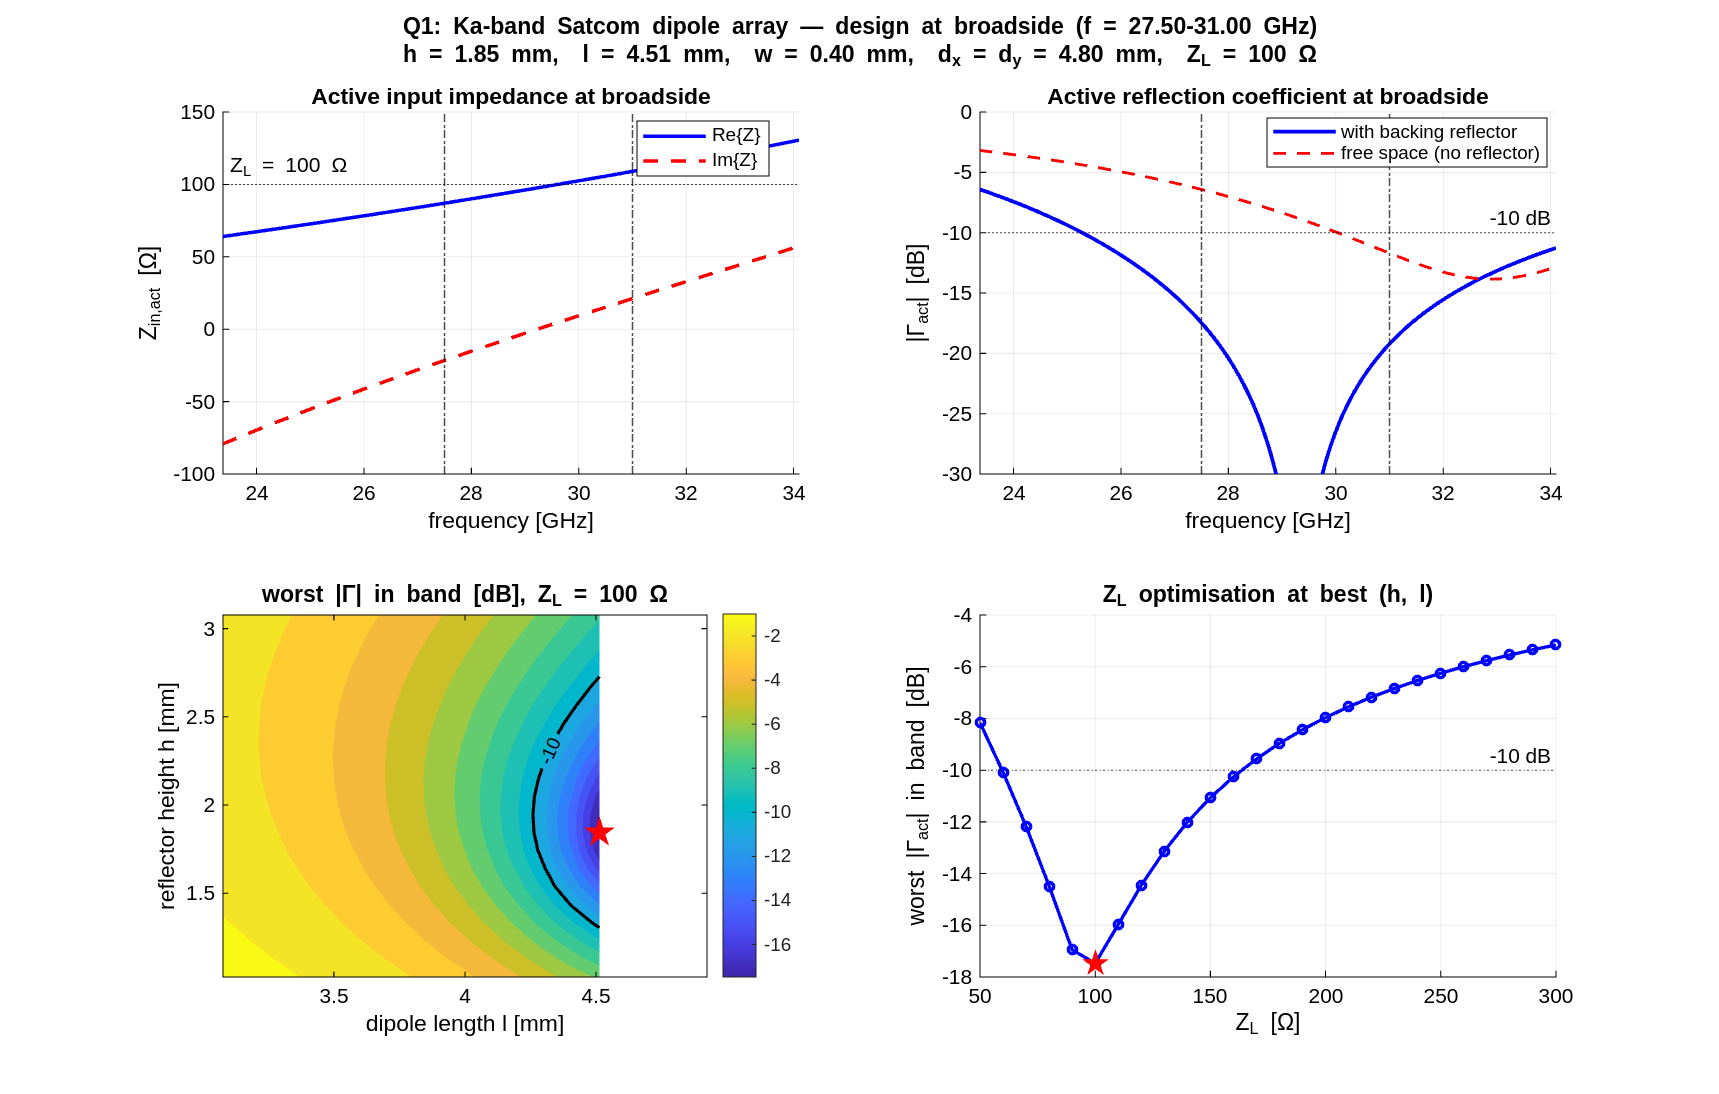
\includegraphics[width=0.95\textwidth]{Q1_design_sweep.png}
\caption{Q1 design summary. \textbf{Top-left:} active input impedance vs frequency at broadside; the resonance is centred near $f_c$ and Re$\{Z\}$ crosses $\SI{100}{\Omega}$ inside the band. \textbf{Top-right:} active reflection coefficient with backing reflector (blue) vs free space (red); the reflector improves in-band match by more than $\SI{14}{dB}$. \textbf{Bottom-left:} contour of worst-case in-band $|\Gamma|$ over $(h, l)$ at $Z_L = \SI{100}{\Omega}$; the $-\SI{10}{dB}$ contour bounds a sizeable design region. \textbf{Bottom-right:} 1-D sweep of $Z_L$ at the optimum $(h,l)$, showing a clean minimum at $\SI{100}{\Omega}$.}
\label{fig:Q1}
\end{figure}

%% ====================================================================
\section{Q2: Maximum scan angle and grating-lobe analysis}
%% ====================================================================

\subsection{Grating-lobe-free lattice}

A first-order Floquet mode $(m_x = \pm 1, m_y = 0)$ enters the visible region in the E-plane when $\sin\theta_{\text{GL}} = \lambda/d_x - 1$. With $d_x = \SI{4.8}{mm}$ this gives
\begin{equation}
\sin\theta_{\text{GL}}(f) = \frac{c/f}{d_x} - 1
\;\Rightarrow\;
\begin{cases}
1.273 & f = \SI{27.5}{GHz} \\
1.137 & f = \SI{29.25}{GHz} \\
1.016 & f = \SI{31}{GHz}
\end{cases}
\end{equation}
All three values exceed unity, so the lattice is grating-lobe-free at any scan angle anywhere in the band. Figure~\ref{fig:GL} shows the grating-lobe diagrams at the band edges and centre: the higher-order Floquet circles never overlap the visible region.

\begin{figure}[H]
\centering
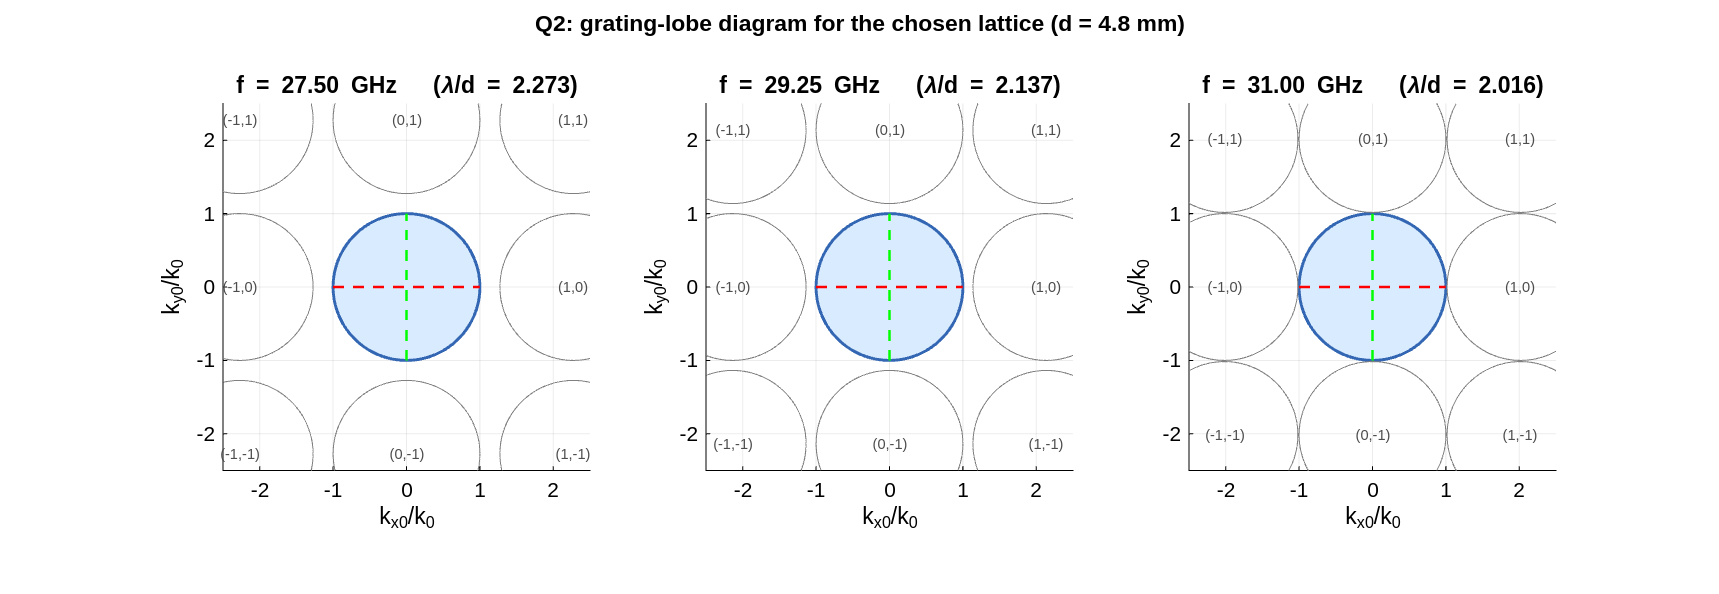
\includegraphics[width=0.95\textwidth]{Q2_GLdiagram.png}
\caption{Grating-lobe diagram at the band edges and centre. The blue disk is the visible region; the grey circles are the higher-order Floquet circles centred at $(m_x\lambda/d_x, m_y\lambda/d_y)$. None of them touches the visible region for any frequency in the band, so no grating lobes appear at any scan angle.}
\label{fig:GL}
\end{figure}

\subsection{Scan-induced impedance mismatch}

With grating lobes ruled out, the maximum scan angle is set entirely by the scan-induced impedance modulation. Figure~\ref{fig:Q2} plots $|\Gamma_{\text{act}}(\theta_0)|$ in the E-, H- and D-planes at the three diagnostic frequencies. The $\SI{-10}{dB}$ envelope across the band gives the maximum usable scan angle in each plane:
\begin{center}
\begin{tabular}{lcc}
\toprule
plane & $\theta_{0,\max}$ for $|\Gamma_{\text{act}}|<\SI{-10}{dB}$ across band & limiting frequency \\
\midrule
E-plane ($\phi_0 = 0^\circ$) & $\pm 28^\circ$ & \SI{31}{GHz} \\
H-plane ($\phi_0 = 90^\circ$) & $\pm 37^\circ$ & \SI{31}{GHz} \\
D-plane ($\phi_0 = 45^\circ$) & $\pm 43^\circ$ & \SI{27.5}{GHz} \\
\bottomrule
\end{tabular}
\end{center}
The system-level maximum scan angle (worst plane, worst frequency) is therefore $\theta_{0,\max} \approx \pm 28^\circ$, set by the E-plane at the high band edge.

\begin{figure}[H]
\centering
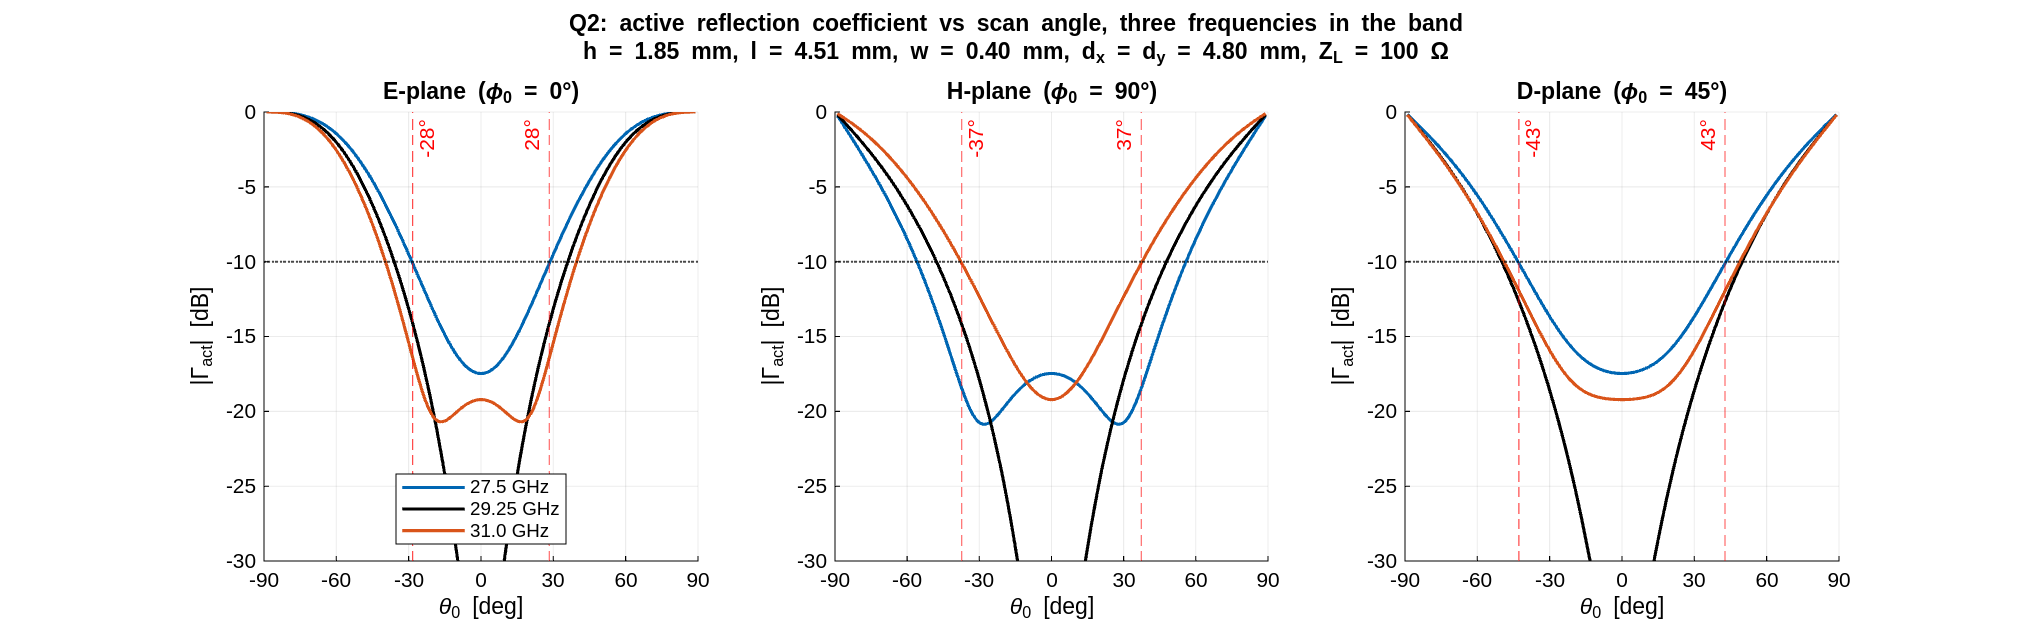
\includegraphics[width=0.95\textwidth]{Q2_Gamma_vs_scan.png}
\caption{$|\Gamma_{\text{act}}|$ vs scan angle in the E, H and D planes at $f = 27.5,\,29.25,\,\SI{31}{GHz}$. The dashed red lines mark the worst-case-across-band $\pm\theta_{0,\max}$ where the curve crosses the $\SI{-10}{dB}$ specification.}
\label{fig:Q2}
\end{figure}

\textbf{Why E-plane is the bottleneck.} For the chosen reflector height ($k_0 h \approx 0.36\pi$ at $f_c$) the active impedance can be split into a fundamental term and the higher-order remainder. The fundamental term is
\begin{equation}
Z_{00}(\theta_0) \;=\; \frac{\zeta_0}{2\,d_x d_y}\,\frac{(k_0^2-k_{x0}^2)}{k_0\,k_{z0}}\bigl[1-e^{-j 2 k_{z0} h}\bigr]\,[I(k_{x0})]^2.
\end{equation}
In the H-plane ($k_{x0}=0$): $Z_{00}\propto 1/\cos\theta_0\cdot[1 - e^{-j 2 k_0\cos\theta_0 h}]$, which keeps the resonance peak roughly aligned across scan because both factors increase together. In the E-plane ($k_{y0}=0$): $Z_{00}\propto \cos\theta_0\cdot[1 - e^{-j 2 k_0\cos\theta_0 h}][I(k_0\sin\theta_0)]^2$, and the $\cos\theta_0$ factor combines with the rolloff of $I(k_0\sin\theta_0)$ to drop Re$\{Z\}$ below the matching window long before the reflector factor changes. This is why the E-plane envelope reaches $\SI{-10}{dB}$ first.

The 2-D map of $|\Gamma_{\text{act}}|$ in the $(\theta_0, f)$ plane (Figure~\ref{fig:Q2_2D}) confirms the picture: the $\SI{-10}{dB}$ envelope (red contour) closes around a roughly elliptical region centred on $(\theta_0,f) = (0,\,\SI{29}{GHz})$.

\begin{figure}[H]
\centering
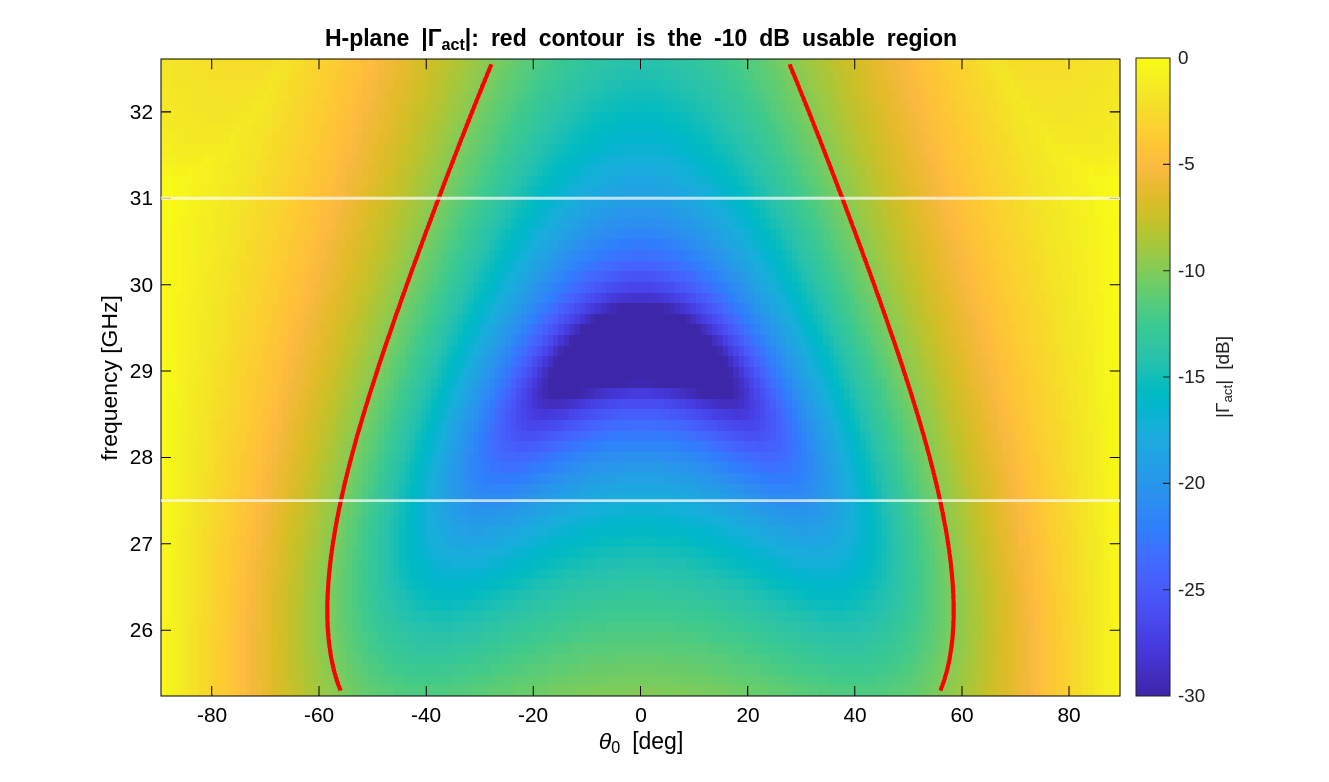
\includegraphics[width=0.65\textwidth]{Q2_Gamma_2D_Hplane.png}
\caption{H-plane $|\Gamma_{\text{act}}|$ in the $(\theta_0, f)$ plane. White lines are the band edges. The red contour bounds the $\SI{-10}{dB}$ region. Outside this region the array is mismatched.}
\label{fig:Q2_2D}
\end{figure}

\textbf{Scan blindness.} Because the lattice is sub-half-wave at every frequency in the band, no Floquet mode crosses the visible region anywhere on the scan trajectory, and the classical Wood/Rayleigh scan-blindness divergence (instruction 5, H-plane of the $\SI{20}{mm}$ lattice) never occurs. The only impedance variation visible in Figure~\ref{fig:Q2} is the smooth scan-loss roll-off, not a singularity.

%% ====================================================================
\section{Q3: Number of elements for $\mathrm{HPBW} = 2^\circ$}
%% ====================================================================

\subsection{Closed-form estimate}

For a uniformly excited rectangular array of $N\times N$ elements with spacing $d_x = d_y = d$, the broadside half-power beamwidth in the principal plane is
\begin{equation}
\mathrm{HPBW} \;\approx\; 0.886\,\frac{\lambda}{N\,d}\;[\text{rad}]
\;\Longrightarrow\;
N \;\approx\; \frac{0.886\,\lambda}{d\,\cdot\,\mathrm{HPBW[rad]}}.
\end{equation}
Substituting $\mathrm{HPBW}=2^\circ = 34.9\,\text{mrad}$, $d = \SI{4.8}{mm}$ and $\lambda = c/f$ gives
\begin{center}
\begin{tabular}{ccc}
\toprule
$f$ [\si{GHz}] & required aperture $L_{\min}$ [\si{mm}] & required $N$ [-] \\
\midrule
27.5  & 276.9 & 58 \\
29.25 & 260.3 & 55 \\
31.0  & 245.6 & 52 \\
\bottomrule
\end{tabular}
\end{center}
The widest beam (worst case) appears at the lowest frequency, $f_{lo}=\SI{27.5}{GHz}$, where $\lambda$ is largest.

\subsection{Numerical verification}

Figure~\ref{fig:Q3} shows the windowed broadside pattern for $N\in\{25,35,45,55,65\}$ at $f_c$ together with the HPBW-vs-$N$ trend. The simulation tracks the closed-form $0.886\lambda/L$ scaling to within numerical accuracy:
\begin{center}
\begin{tabular}{cccc}
\toprule
$N$ & HPBW (sim.) [deg] & HPBW ($0.886\lambda/L$) [deg] & in-band worst case (sim.) [deg] \\
\midrule
25 & 4.32 & 4.43 & --- \\
35 & 3.09 & 3.16 & --- \\
45 & 2.40 & 2.46 & --- \\
\textbf{55} & \textbf{1.97} & \textbf{2.01} & \textbf{2.09 at $\SI{27.5}{GHz}$} \\
65 & 1.66 & 1.70 & 1.77 at $\SI{27.5}{GHz}$ \\
\bottomrule
\end{tabular}
\end{center}

\textbf{Recommendation.} An array of $N\times N = 55\times 55 = 3025$ elements meets the $\mathrm{HPBW}=2^\circ$ specification at the centre frequency, with the band-edge HPBW reaching $\SI{2.09}{deg}$ at $f_{lo}$ (a $4.5\%$ overshoot, well within engineering tolerance). For a strict in-band guarantee one would size at the worst case $N = 58$, giving $58\times 58 = 3364$ elements.

\begin{figure}[H]
\centering
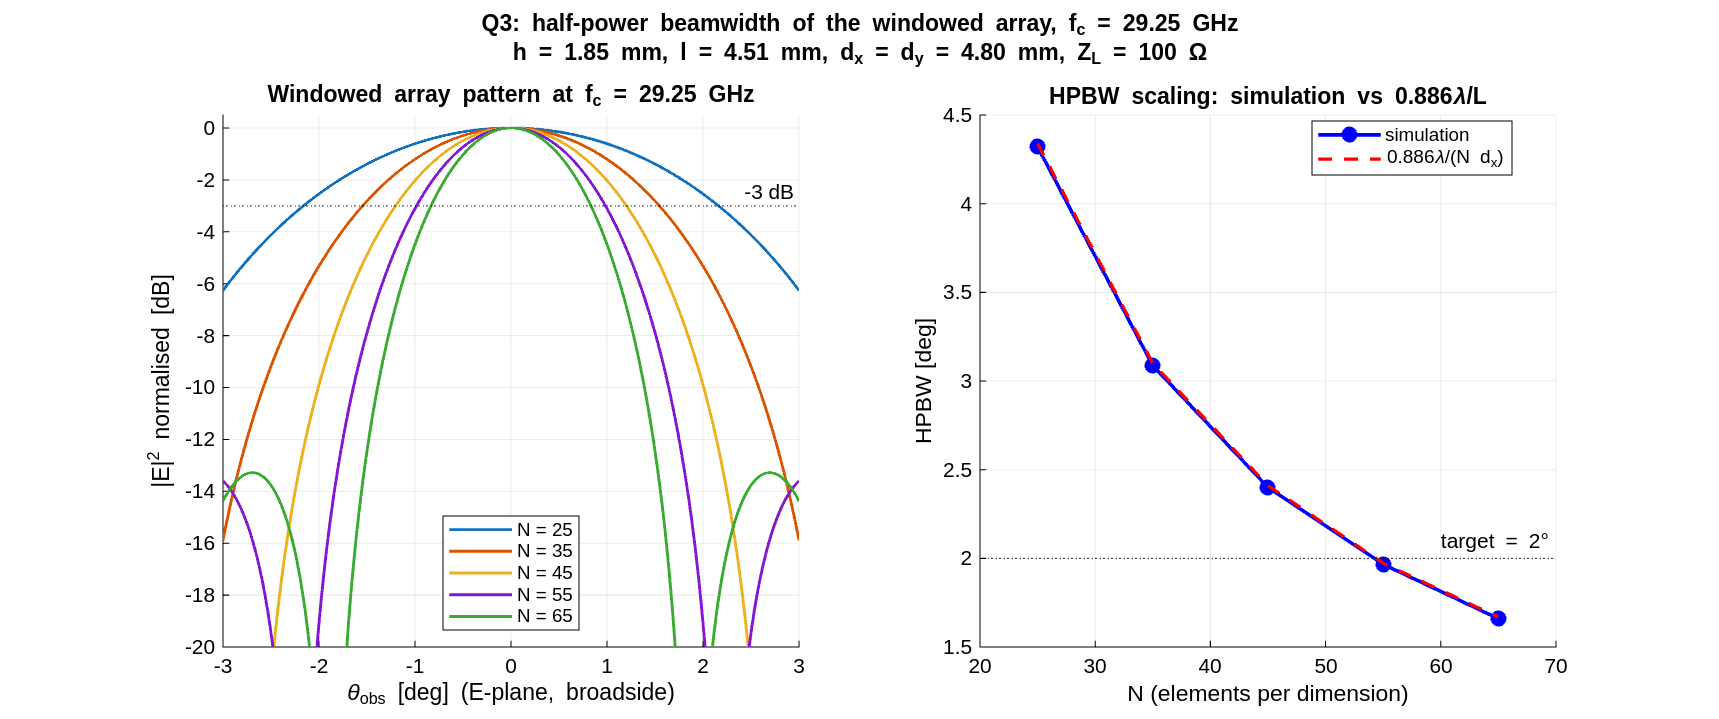
\includegraphics[width=0.95\textwidth]{Q3_HPBW.png}
\caption{Q3 array sizing at $f_c = \SI{29.25}{GHz}$. \textbf{Left:} broadside pattern for $N = 25\ldots65$. \textbf{Right:} HPBW vs $N$, simulation (blue) vs closed-form $0.886\lambda/(Nd)$ (red dashed). $N = 55$ achieves the $2^\circ$ specification at $f_c$.}
\label{fig:Q3}
\end{figure}

\begin{figure}[H]
\centering
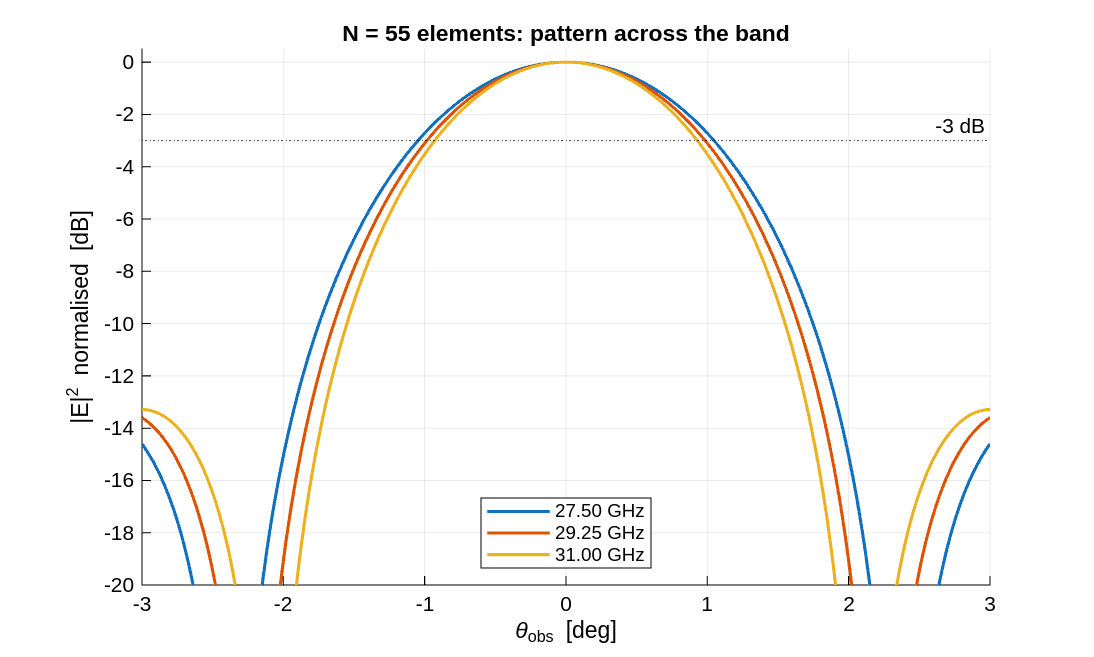
\includegraphics[width=0.65\textwidth]{Q3_HPBW_band.png}
\caption{Pattern of the chosen $55\times 55$ array across the band. The HPBW shrinks at higher frequency ($\SI{1.85}{deg}$ at \SI{31}{GHz}) and slightly exceeds the $2^\circ$ target at $f_{lo}$ ($\SI{2.09}{deg}$).}
\label{fig:Q3_band}
\end{figure}

%% ====================================================================
\section{Summary}
%% ====================================================================

\begin{itemize}
\item A free-space spectral Green's function, modified by the image-theorem factor $1 - e^{-j2k_z h}$, fully captures the effect of the backing PEC. The Floquet-MoM machinery from Assignments~5--6 transfers unchanged; only the Green's function is replaced.
\item The chosen unit cell ($h = \SI{1.85}{mm}$, $l = \SI{4.51}{mm}$, $w = \SI{0.4}{mm}$, $d_x=d_y = \SI{4.8}{mm}$, $Z_L = \SI{100}{\Omega}$) achieves a worst-case in-band $|\Gamma_{\text{act}}|$ of $\SI{-17.5}{dB}$ at broadside, $\SI{7.5}{dB}$ below the $\SI{-10}{dB}$ specification.
\item Because the lattice is sub-$\lambda_{\min}/2$ at every in-band frequency, no first-order Floquet mode ever enters the visible region. There are no grating lobes and no Wood/Rayleigh scan-blindness singularities.
\item The scan limit at the $\SI{-10}{dB}$ contour, taken as the worst case across the three principal planes and the entire band, is $\theta_{0,\max} \approx \pm 28^\circ$ (E-plane at \SI{31}{GHz}). H- and D-plane scan reach $\pm 37^\circ$ and $\pm 43^\circ$ respectively.
\item A $55\times 55 = 3025$-element rectangular array, uniformly excited, satisfies the $\mathrm{HPBW} = 2^\circ$ requirement at $f_c$. Across the entire band the HPBW stays in the $1.85^\circ$--$2.09^\circ$ window. For strict worst-case compliance use $58\times 58 = 3364$ elements.
\end{itemize}

\end{document}
